\section{Background from specific decays}

A survey of possible peaking backgrounds concluded that the only physics background
to take into account is coming from misreconstructed decays of \Bz to \KS with
two muons, whether via \jpsi or not. The lack of background from other decays is
mainly due to the particular topology of the \Lz decay which has a displaces vertex.
%This can in principle affect both rare and \jpsi channels.
In order to study the effect of misreconstructed $\Bz\ra\jpsi\KS$ and $\Bz\ra\KS\mumu$ decays
simulated samples are used, where the \KS is reconstructed as a \Lz with a $p\rightarrow \pi$ identity
swap and $m(p\pi)$ in the \Lz mass window.
On data the $\Bz\ra\jpsi\KS$ contribution is clearly visible in the resonant channel mass distribution.
This background is not suppressed with specific cuts in this analysis as its mass shape is sufficiently distinct
the from \Lb signal, which allows to reliably model its contribution in the mass fits (see Sec.~\ref{sec:Lb_fit}).
For rare case a rough estimate of the size is made using the yield in the resonant channel
rescaled the measured ratios between the rare and resonant branching ratios. 
Details are given in Sec.~\ref{sec:Lb_fit} and numbers of events predicted are reported in Tab.~\ref{tab:KSprediction}.
This contribution, although close to negligible is again considered in the fit.
A possible pollution due to $B^{+} \ra\mumu K^{*+}$ decays, where the $K^{*+}$
further decays into $\KS\pi$ is also investigated using a dedicated Monte Carlo sample and found to be negligible.
Finally, $\Lb\ra\jpsi\Lz$ events radiating photons from the final state, can escape the \jpsi veto
and be reconstructed in the rare channel. The only contribution observed using simulated $\Lb\ra\jpsi\Lz$ events ends up
in the interval just below the \jpsi exclusion region, between 7 and 8 \gevcc in \qsq.
Given that this contribution does not contribute in the region where we expect \Lb peak, we do
not attempt to exclude this but it is again modelled in the fit.
In Fig.~\ref{fig:peakingBkgs} is reported the invariant mass distribution of simulated $\Lb\ra\jpsi\Lz$
events falling into the rare \qsq region.
                          

\begin{figure}
\centering
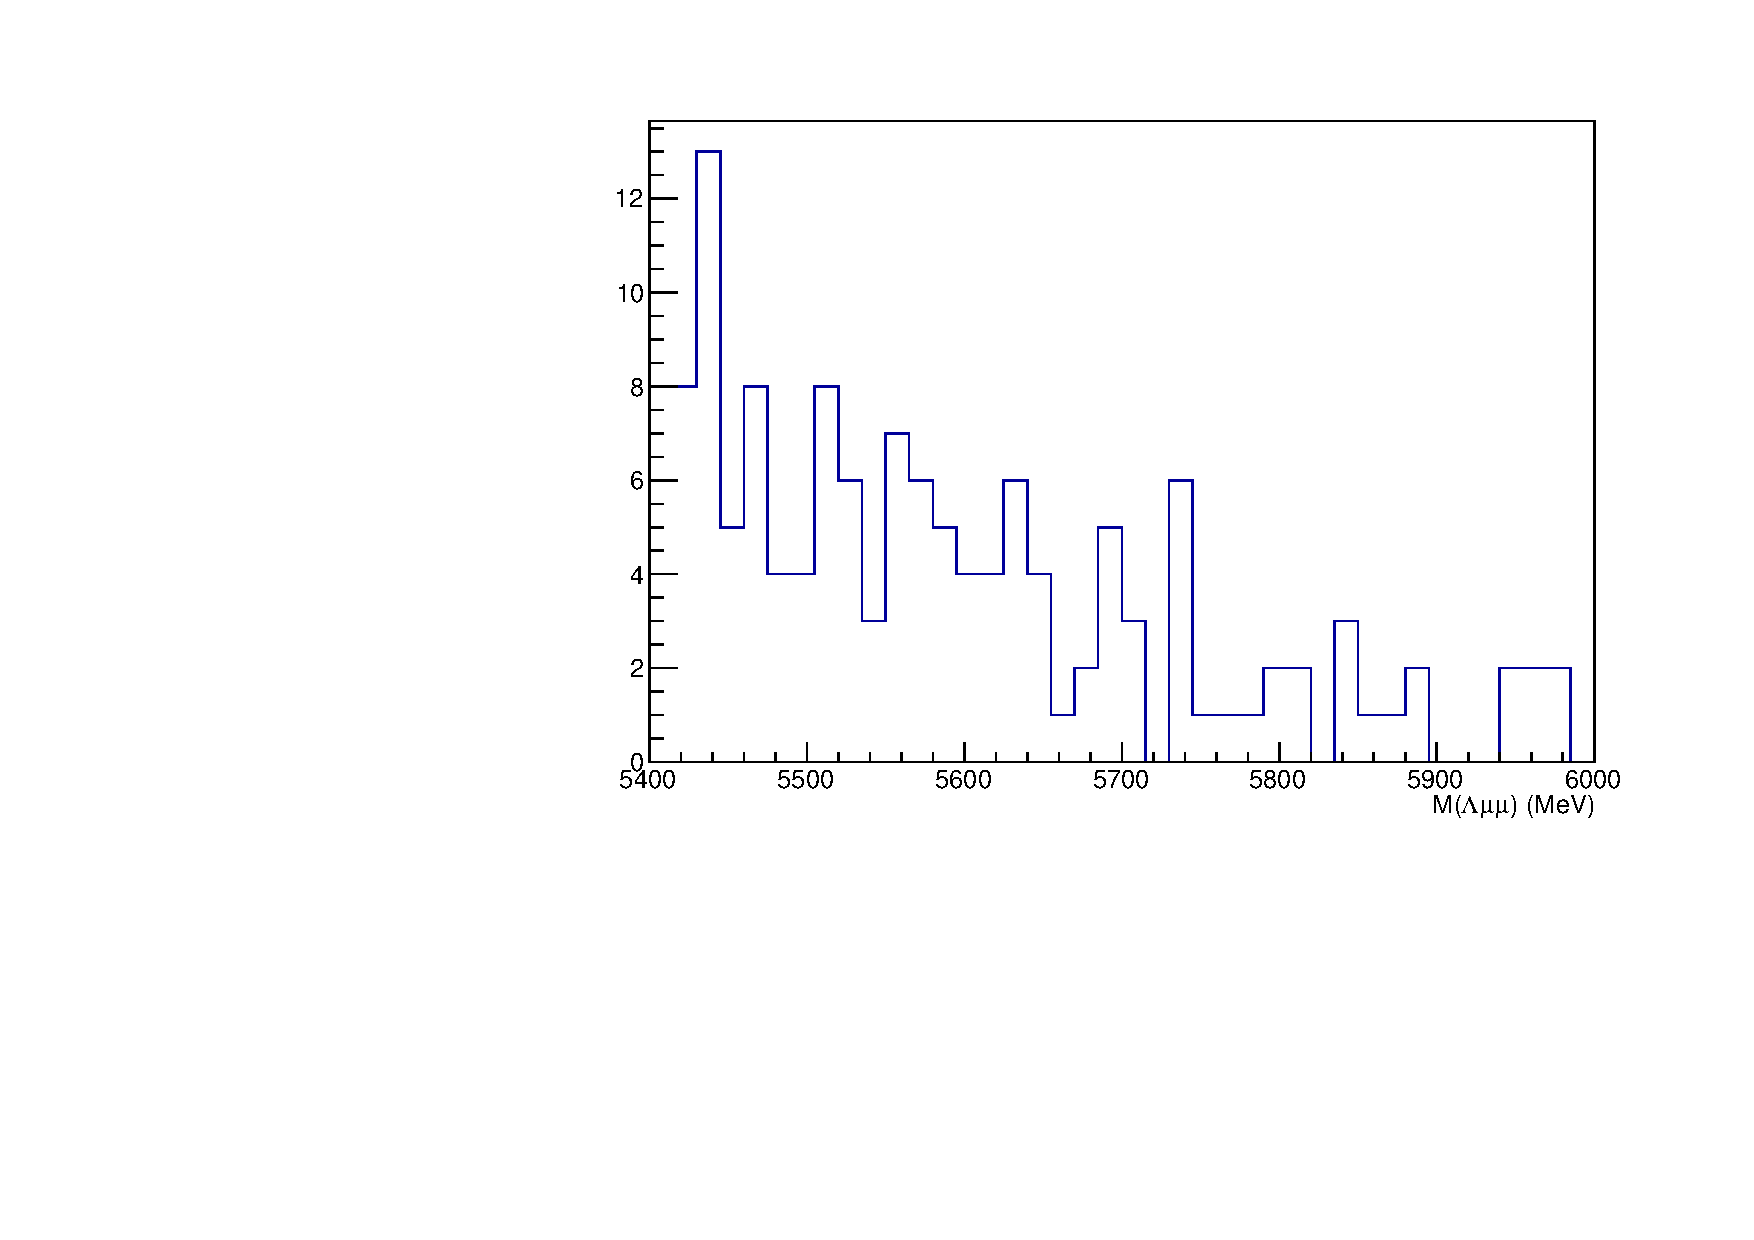
\includegraphics[width=0.48\textwidth]{Lmumu/figs/Kst_plus_distrib.pdf}
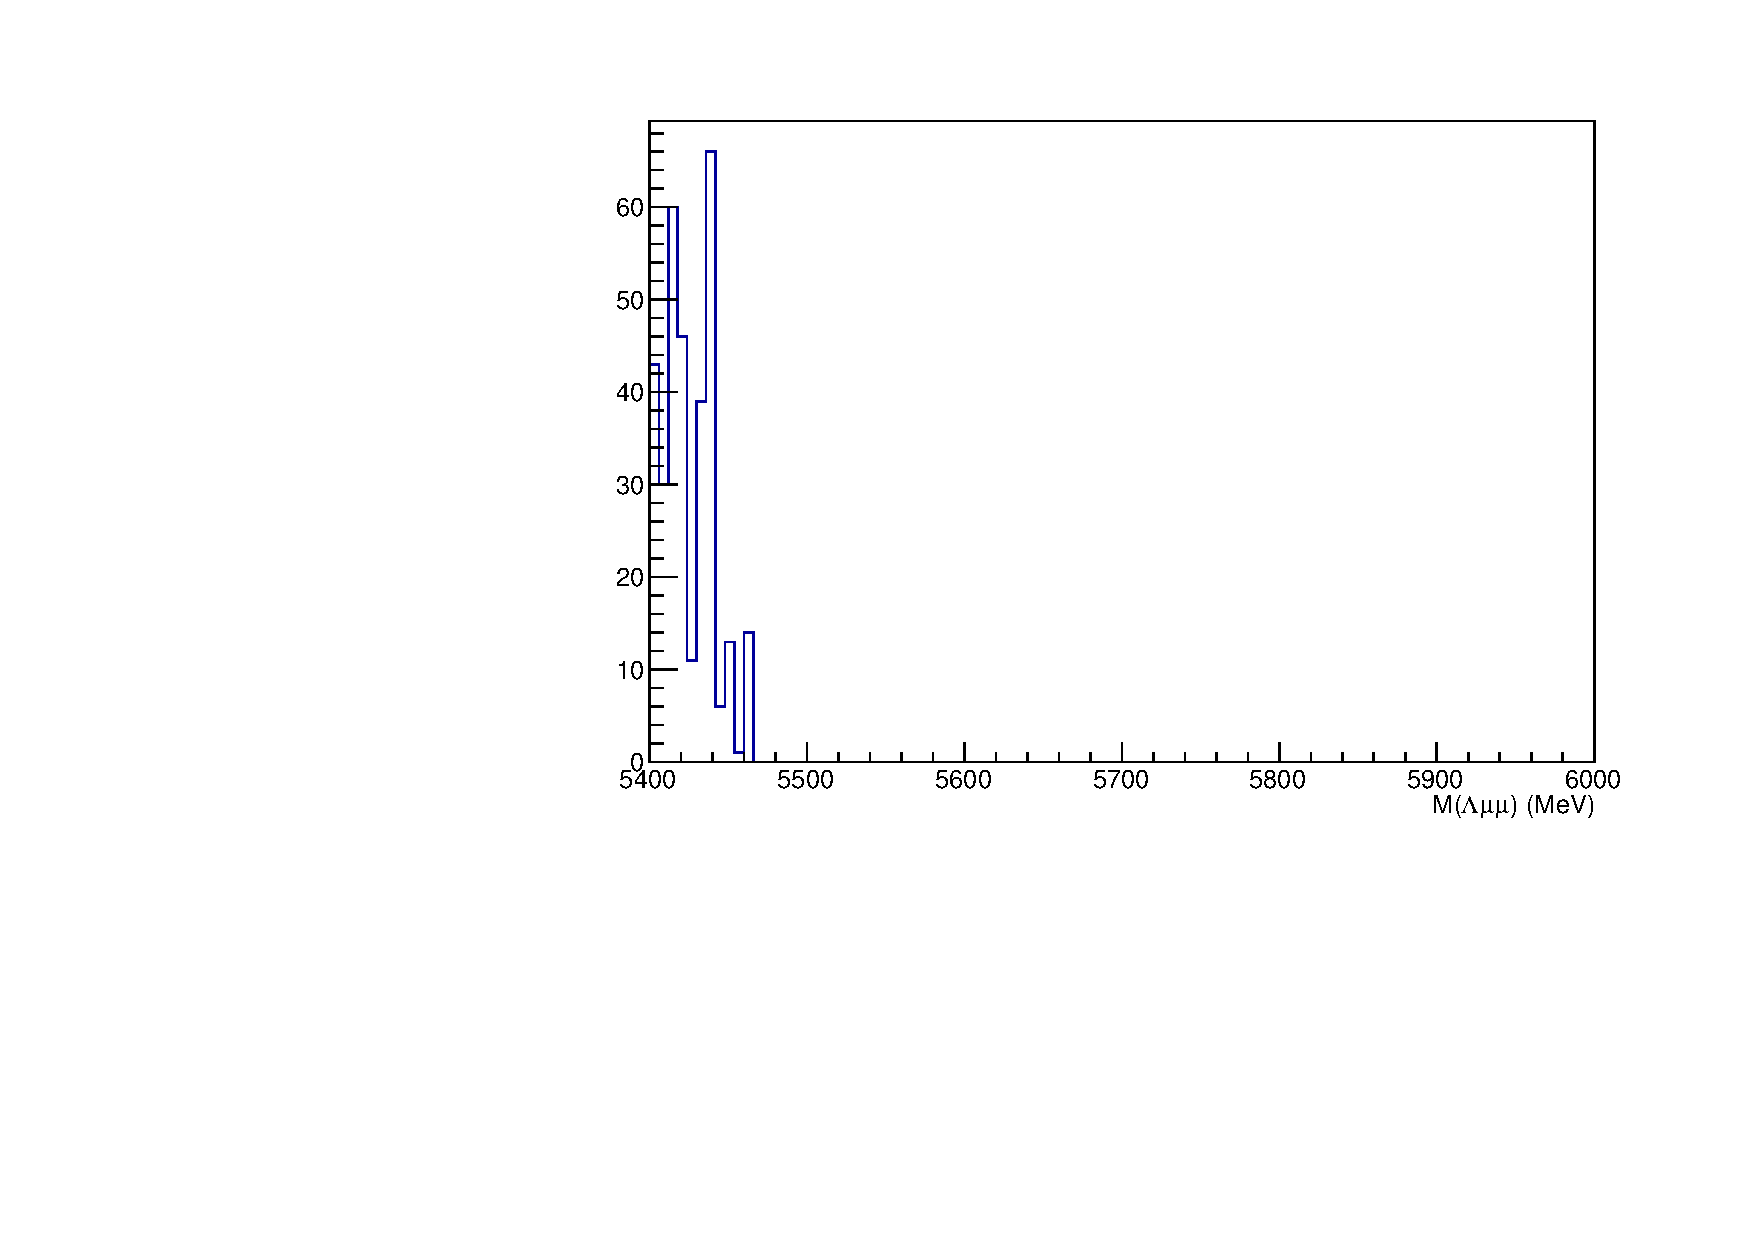
\includegraphics[width=0.48\textwidth]{Lmumu/figs/Jpsi_tail_distrib.pdf}
\caption{ Inariant mass distribution of fully slected $B^{+} \ra\mumu K^{*+}$ MC events (left)
and of generator level events from \jpsi radiative tail in the region $\qsq < 8$ \gevgevcccc (right). }
\label{fig:peakingBkgs}
\end{figure}

